\documentclass[10pt]{standalone}
%\usepackage[utf8]{inputenc}
\usepackage{pgfplots}
\pgfplotsset{compat=1.15}
\usepackage{mathrsfs}
\usetikzlibrary{arrows}
\pagestyle{empty}
\begin{document}
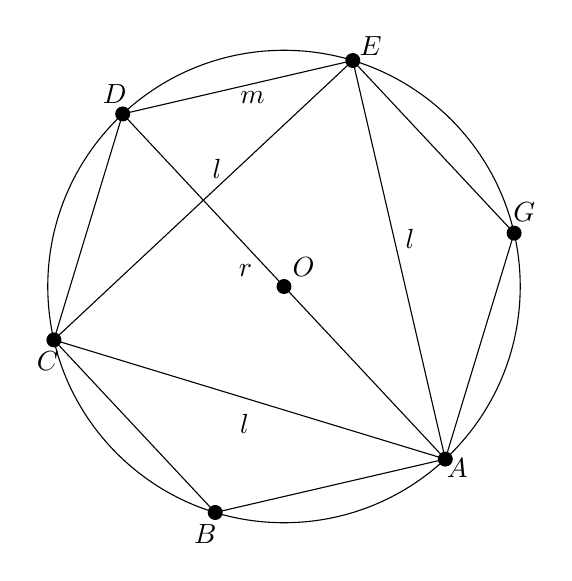
\begin{tikzpicture}[line cap=round,line join=round,>=triangle 45,x=0.5cm,y=0.5cm]

%\clip(-2.5,-3.5) rectangle (10.5,9.5);
\draw  (4.,3.) circle (3.cm);
\draw  (5.747612254333397,8.73984768164659)-- (9.844660033325862,4.356447232605583);
\draw  (9.844660033325862,4.356447232605583)-- (8.097047778992465,-1.3834004490410088);
\draw  (8.097047778992465,-1.3834004490410088)-- (2.2523877456666037,-2.739847681646591);
\draw  (2.2523877456666037,-2.739847681646591)-- (-1.8446600333258607,1.643552767394417);
\draw  (-1.8446600333258607,1.643552767394417)-- (-0.09704777899246486,7.383400449041006);
\draw  (-0.09704777899246486,7.383400449041006)-- (5.747612254333397,8.73984768164659);
\draw  (5.747612254333397,8.73984768164659)-- (-1.8446600333258607,1.643552767394417);
\draw  (-1.8446600333258607,1.643552767394417)-- (8.097047778992465,-1.3834004490410088);
\draw  (8.097047778992465,-1.3834004490410088)-- (5.747612254333397,8.73984768164659);
\draw  (-0.09704777899246486,7.383400449041006)-- (8.097047778992465,-1.3834004490410088);
\draw [fill=black] (4.,3.) circle (2.5pt);
\draw[color=black] (4.5,3.5) node {$O$};
%\draw[color=black] (1.1053954857516932,7.627162513723629) node {$c$};
\draw [fill=black] (8.097047778992465,-1.3834004490410088) circle (2.5pt);
\draw[color=black] (8.4,-1.6) node {$A$};
\draw [fill=black] (2.2523877456666037,-2.739847681646591) circle (2.5pt);
\draw[color=black] (2.0,-3.3) node {$B$};
\draw [fill=black] (-1.8446600333258607,1.643552767394417) circle (2.5pt);
\draw[color=black] (-2.0,1.1) node {$C$};
\draw [fill=black] (-0.09704777899246486,7.383400449041006) circle (2.5pt);
\draw[color=black] (-0.3,7.9) node {$D$};
\draw [fill=black] (5.747612254333397,8.73984768164659) circle (2.5pt);
\draw[color=black] (6.2,9.1) node {$E$};
\draw [fill=black] (9.844660033325862,4.356447232605583) circle (2.5pt);
\draw[color=black] (10.1,4.9) node {$G$};

\draw[color=black] (3.2,7.8) node {$m$};
\draw[color=black] (2.3,6.0) node {$l$};
\draw[color=black] (3.0,-0.5) node {$l$};
\draw[color=black] (3.0229084878973276,3.4) node {$r$};
\draw[color=black] (7.2,4.2) node {$l$};
\end{tikzpicture}
\end{document}